\NeedsTeXFormat{LaTeX2e}

\documentclass[a4paper,12pt]{pkg/monografia}
\usepackage[pdfpagelabels]{hyperref}
\usepackage{amsmath,amsthm,amsfonts,amssymb}
\usepackage[mathcal]{eucal}
\usepackage{latexsym}
%\usepackage[utf8]{inputenc}
\usepackage[brazil]{babel}
%\usepackage{bm}
\usepackage[alf]{pkg/abntex2cite}
\usepackage{url}
\usepackage{enumitem}
\usepackage{graphicx}
\usepackage{placeins}
%\usepackage{epstopdf}
\usepackage{multirow}
%\usepackage{fancyhdr}
\usepackage[FIGTOPCAP]{subfigure}
\usepackage{textcase}
\usepackage{tabularx}
\usepackage[table,xcdraw]{xcolor}
%\usepackage[portuguese,noend,ruled]{algorithm2e}
\usepackage{listings}
\usepackage[T1]{fontenc}
\usepackage{courier}
\usepackage[printonlyused]{acronym}
\usepackage{caption}
\usepackage{adjustbox}
\usepackage{floatrow}
\floatsetup[figure]{capposition=top}
\floatsetup[table]{capposition=top}
%\captionsetup{labelsep=endash}
%\usepackage{rotating}
%\usepackage{rotfloat}
%\usepackage{placeins}
\usepackage{fontspec}
\setmonofont{Inconsolata}
%\captionsetup[listing]{position=top}

%-----------------------------------------------------------
\begin{document}

%----------------- Título e Dados do Autor -----------------
%\titulo{Análise de arquiteturas de microsserviços empregados a jogos MMORPG voltada a otimização do uso de recursos de gerenciamento de mundos virtuais}
\titulo{Análise de disponibilidade utilizando Docker Swarm}
\autor{Gustavo José Neves da Silva\\Marlon Henry Schweigert}
%\nome{Marlon Henry}
%\ultimonome{Schweigert}

%---------- Informe o Curso e Grau -------------------------
\bacharelado \curso{Ciência da Computação} \mes{Junho} \ano{2018}
\data{\today} % Data da aprovação
\cidade{Joinville}

%---------- Informações sobre a Institução -----------------
\instituicao{Universidade do Estado de Santa Catarina}
\sigla{UDESC} \unidadeacademica{Centro de Ciências Tecnológicas}

%-- Nomes do Orientador, 1o. Examinador e 2o. Examinador ---
\orientador{Charles Christian Miers}
\examinadorum{}
\examinadordois{}
\examinadortres{}

%-- Títulos do Orientador, 1o. Examinador e 2o. Examinador -
\ttorientador{Doutor}
\ttexaminadorum{}
\ttexaminadordois{}
\ttexaminadortres{}

%---------- Capa -------------------------------------------
\maketitle

%---------- Agradecimentos----------------------------------
%\agradecimento{Agradecimentos}
\section*{Agradecimentos}

AGRADECIMENTOS

%\newpage

%---------- Epígrafe ---------------------------------------
%\begin{epigrafe}



%\end{epigrafe}

%---------- Resumo -----------------------------------------
\resumo{Resumo}
A crescente popularização de jogos massivos demanda por novas abordagens tecnológicas a fim de suprir as necessidades dos usuários com menor custo de recursos computacionais.
%
Projetar essas arquiteturas, do ponto de vista da rede, é algo pertinente e impactante para o sucesso desses jogos.
%
O objetivo deste trabalho é propor uma análise voltada a identificar abordagens para otimização dos recursos computacionais consumidos pelas arquiteturas identificadas.
%
Esse objetivo será atingido após realizar uma pesquisa referenciada, seguida de uma análise das principais arquiteturas e, preferencialmente, a execução de simulações usando uma nuvem computacional para auxiliar na identificação de gargalos de recursos. Os resultados obtidos auxiliarão provedores de serviços \ac{mmorpg} a reduzir gastos de manutenção e melhorar a qualidade de tais serviços.

\\
\noindent \textbf{Palavras-chaves:} Arquitetura de microsserviços, Docker, Docker Swarm

%---------- Abstract ---------------------------------------
%\resumo{Abstract}
%Lorem ipsum dolor sit amet, consectetur adipisicing elit, sed do eiusmod tempor incididunt ut labore et dolore magna aliqua. Ut enim ad minim veniam, quis nostrud exercitation ullamco laboris nisi ut aliquip ex ea commodo consequat. Duis aute irure dolor in reprehenderit in voluptate velit esse cillum dolore eu fugiat nulla pariatur. Excepteur sint occaecat cupidatat non proident, sunt in culpa qui officia deserunt mollit anim id est laborum.

%\\
%\noindent \textbf{Keywords:} Microservices Arquiteture, Docker, Docker Swarm
%-----------------------------------------------------------

% SUMÁRIO, LISTA DE FIGURAS E LISTA DE TABELAS
%---------- Sumário ----------------------------------------
\tableofcontents
\thispagestyle{empty}

%---------- Lista de figuras -------------------------------
\listoffigures
\thispagestyle{empty}

%---------- Lista de tabelas -------------------------------
\listoftables
\thispagestyle{empty}

%---------- Lista de Abreviaturas --------------------------
\listofabbreviations{Lista de Abreviaturas}
\begin{acronym}[]
	\acro{amqp}[AMQP]{{\it Advanced Message Queuing Protocol}}
	\acro{api}[API]{{\it Application Programming Interface}}
  \acro{aws}[AWS]{{\it Amazon Web Services}}
	\acro{cli}[CLI]{{\it Command Line Interface}}
	\acro{cpu}[CPU]{{\it Central Processing Unit}}
	\acro{crud}[CRUD]{{\it Create Read Update Delete}}
	\acro{cs}[C/S]{{Cliente/Servidor}}
	\acro{ddos}[DDoS]{{\it Distributed Denial of Service}}
	\acro{fps}[FPS]{{\it First-person shooter}}
	\acro{http}[HTTP]{{\it Hypertext Transfer Protocol}}
	\acro{iaas}[IaaS]{{\it Infrastructure as a Service}}
  \acro{ids}[IDS]{{\it Intrusion Detection System}}
	\acro{json}[JSON]{{\it JavaScript Object Notation}}
	\acro{jwt}[JWT]{{\it JSON Web Token}}
	\acro{kvm}[KVM]{{\it Kernel-based Virtual Machine}}
	\acro{lan}[LAN]{{\it Local Area Network}}
  \acro{ldap}[LDAP]{{\it Lightweight Directory Access Protocol}}
	\acro{mhz}[MHz]{{\it Mega-hertz}}
	\acro{mmo}[MMO]{{\it Massively Multiplayer Online}}
	\acro{mmofps}[MMOFPS]{{\it Massively Multiplayer Online First-Person Shooter}}
	\acro{mmorpg}[MMORPG]{{\it Massively Multiplayer Online Role-Playing Game}}
	\acro{moba}[MOBA]{{\it Multiplayer Online Battle Arena}}
	\acro{mvc}[MVC]{{\it Model-View-Controller}}
	\acro{nist}[NIST]{{\it National Institute of Standards and Technology}}
	\acro{npcs}[NPCs]{{\it Non-Playable Characters}}
	\acro{ntsc}[NTSC]{{\it National Television System Committee}}
	\acro{p2p}[P2P]{{\it Peer-to-peer}}
	\acro{pvp}[PvP]{{\it Player vs Player}}
	\acro{pvnpc}[PvNPCs]{{\it Player vs \ac{npcs}}}
	\acro{paas}[PaaS]{{\it Platform as a Service}}
	\acro{pov}[POF]{{\it Point of View}}
	\acro{qos}[QoS]{{\it Quality of Service}}
	\acro{ram}[RAM]{{\it Random Access Memory}}
	\acro{rest}[REST]{{\it Representational State Transfer}}
	\acro{rpc}[RPC]{{\it Remote Procedure Call}}
	\acro{rpg}[RPG]{{\it Role-Playing Game}}
	\acro{rts}[RTS]{{\it Real-Time Strategy}}
	\acro{sdn}[SDN]{{\it Software Defined Network}}
	\acro{saas}[SaaS]{{\it Software as a Service}}
	\acro{snmp}[SNMP]{{\it Simple Network Management Protocol}}
	\acro{tcp}[TCP]{{\it Transmission Control Protocol}}
	\acro{tps}[TPS]{{\it Third-person Shooter}}
	\acro{tia}[TIA]{{\it Television Interface Adapter}}
	\acro{udp}[UDP]{{\it User Datagram Protocol}}
	\acro{vlan}[VLAN]{{\it Virtual Local Area Network}}
	\acro{vm}[VM]{{\it Virtual Machine}}
	\acro{vpn}[VPN]{{\it Virtual Private Network}}
	\acro{wan}[WAN]{{\it Wide Area Network}}
	\acro{ws}[WS]{{\it Web Services}}
	\acro{xml}[XML]{{\it Extensible Markup Language}}



	\acrodefplural{vpn}[VPNs]{{\it Virtual Private Networks}}
	\acrodefplural{vlan}[VLANs]{{\it Virtual Local Area Networks}}
	\acrodefplural{vm}[VMs]{{\it Virtual Machines}}
\end{acronym}

% Defining: \acro{acronym}[short name]{full name}
% Usaging:
% \ac{acronym}     -- writes the full name followed by the acronym in brackets; later calls will write only the acronym
% \acf{acronym}     -- writes the full name followed by the acronym in brackets
% \acs{acronym}     -- writes the short name only
% \acl{acronym}     -- writes the full name only
% Use p at the end of previous commands for plural form (e.g., \acp for the plural form of \ac)
% \acresetall        -- reset usage of all acronyms (i.e., \ac will print full name again)
% \acused                -- mark the acronym as used

\thispagestyle{empty}

%---------- Início do Conteúdo -----------------------------
\pagestyle{ruledheader}

\chapter{Introdução}
\label{cap1}


\section{Fundamentação Teórica}


A fim de orientar o análise encontrada neste trabalho, se faz necessário a descrição e pesquisa por fundamentação teórica dos conceitos básicos relevantes no contexto de microsserviços e implantação dessas arquiteturas.
%
Por esse motivo, esta seção irá introduzir os conceitos de microsserviços, containers, docker e implantação utilizando a técnica de docker swarm.


\subsection{Microserviços: Definição e Funcionamento}

Entende-se por microsserviço, aplicações que executam operações menores de um macrosserviço, da melhor forma possível~\cite{stephenclarkewillson2017, Newman2015Feb}.
%
O objetivo de uma arquitetura de microsserviços é funcionar separadamente de forma autônoma, contendo baixo acoplamento~\cite{Newman2015Feb}.
%
Seu funcionamento deve ser desenhado para permitir alinhamentos de alta coesão e baixo acoplamento entre os demais microsserviços existentes em um macrosserviço~\cite{8169955}.



Arquiteturas de microsserviços iniciam uma nova linha de desenvolvimento de aplicações preparadas para executar sobre nuvens computacionais, promovendo maior flexibilidade, escalabilidade, gerenciamento e desempenho, sendo a principal escolha de arquitetura de grandes empresas como Amazon, Netflix e LinkedIn~\cite{7830692,7515686}.
%
Um microsserviço é definido pelas seguintes características~\cite{8169955}:



\begin{itemize}
  \item Deve possibilitar a implementação como uma peça individual do macrosserviço.
  \item Deve funcionar individualmente.
  \item Cada serviço deve ter uma interface. Essa interface deve ser o suficiente para utilizar o microsserviço.
  \item A interface deve estar disponível na rede para chamada de processamento remoto ou consulta de dados.
  \item O serviço pode ser utilizado por qualquer linguagem de programação e/ou plataforma.
  \item O serviço deve executar com as dependências mínimas.
  \item Ao agregar vários microsserviços, o macrosserviço resultante poderá prover funcionalidades complexas.
\end{itemize}



O microsserviço deverá ser uma entidade separada.
%
A entidade deve ser implantada como um sistema independente em um \ac{paas}.
%
Toda a comunicação entre os microsserviços de um macrosserviço será executada sobre a rede, a fim de reforçar a separação entre cada serviço.
%
As chamadas pela rede com o cliente ou entre os microsserviços será executada através de uma \ac{api}, permitindo a liberdade de tecnologia em que cada um será implementado~\cite{Newman2015Feb}.
%
Isso permite que o sistema contenha tecnologias distintas que melhor resolvam os problemas relacionados ao contexto deste microsserviço.
%
Isso pode ser visualizado na Figura~\ref{fig:microsservicos_tecnologias}.



\begin{figure}[htb!]
\caption{Microsserviços podem ter diferentes tecnologias}
\label{fig:microsservicos_tecnologias}
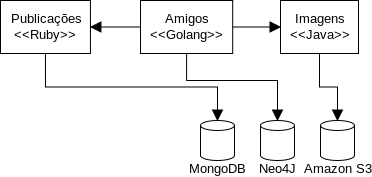
\includegraphics[height=4cm]{img/cap2/microsservicos_tecnologias.png}
\centering

Adaptado de:~\cite{Newman2015Feb}
\end{figure}



Uma arquitetura de microsserviços é escalável, como visível na Figura \ref{fig:microsservicos_escalabilidade}.
%
Ela permite o aumento do número de microsserviços sob demanda para suprir a necessidade de escalabilidade.
%
Este modelo computacional obtém maior desempenho, principalmente se executar sobre plataformas de computação elástica, na qual o orquestrador do macrosserviço pode aumentar o número de instâncias conforme a necessidade de requisições~\cite{Nadareishvili2016Aug}.



\begin{figure}[htb!]
\caption{Microsserviços são escaláveis}
\label{fig:microsservicos_escalabilidade}
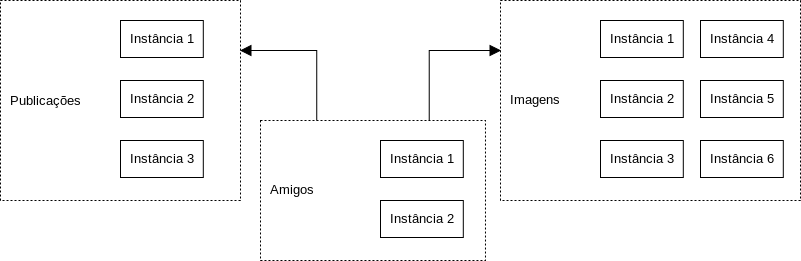
\includegraphics[height=5cm]{img/cap2/microsservicos_escalabilidade.png}
\centering

Adaptado de:~\cite{Newman2015Feb}
\end{figure}



Microsserviços desenvolvidos para web utilizam arquitetura \ac{rest} baseado sobre o protocolo \ac{http}.
%
É uma boa prática utilizar o corpo com conteúdo da requisição e resposta no formato \ac{json} nas chamadas a uma \ac{api} de microsserviço web~\cite{Nadareishvili2016Aug}.

Entretanto, necessita-se de um método para garantir o seu isolamento, a qual, em sistemas Linux, podem ser garantidos utilizando Containers.
%
Por este motivo, se faz necessário descreve-lo.



\subsection{Containers}



Os container permitem ao desenvolvedor "empacotar" sua aplicação e todas as suas dependências(ex. bibliotecas), dessa forma, lhe é garantido que a aplicação terá o mesmo comportamento independentemente do hospedeiro Linux.

Um container Linux é um conjunto de processos que executam de forma isolada do restante do sistema. Esses processos utilizam arquivos providos de uma imagem, a qual lhe garante a compatibilidade a fim de evitar problemas de versionamento e conflitos de processos.
%
Essa separação pode ser visualizada na Figura~\ref{fig:container}.



\begin{figure}[htb!]
\caption{Containers sobre sistema linux}
\label{fig:container}
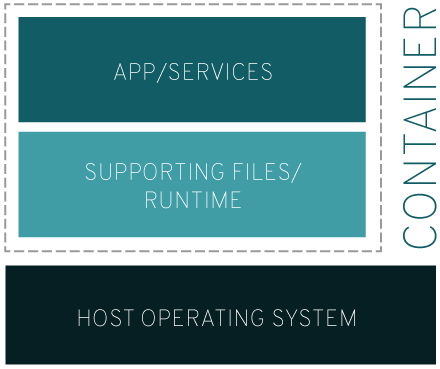
\includegraphics[height=4cm]{img/cap2/what-is-a-container.png}
\centering

Fonte:~\cite{container}
\end{figure}



Entretanto, se faz necessário uma ferramenta para gerenciamento de imagens e containers.
%
Entra em cena a partir de 2008 o \textit{Docker}, uma ferramenta que permite, de forma prática, a publicação de imagens no formato Dockerfile, além de contar com um gerenciador e repositório de imagens.


\subsection{Docker}

Docker é uma plataforma que nos permite "construir, emabarcar e rodar uma aplicação em qualquer lugar". Ele percorreu um longo caminho em um período de tempo incrivelmente curto e atualmente é considerado uma solução padrão para um dos apectos mais custosos do software: a implantação
~\cite{miellJan16}

Docker é uma ferramenta desenvolvida para facilitar o processo de criação, implantação e execução de aplicações por meio do uso de containers.
%
Pode ser pensado como um tipo de maquina virtual, porém diferentemente desta que necessita a criação de todo um sistema operacional virtual, o Docker, permite que as aplicações compartilhem o mesmo kernel Linux que o hospedeiro, reduzindo assim o tamanho da aplicação e obtendo um ganho de desempenho.


A tecnologia Docker usa o \textit{kernel} Linux, abstraindo sistemas como \textit{Cgroups} e \textit{namespaces} para segregar processos a fim que eles possam ser executados de forma independente.
%
O objetivo dos containers criados pelo Docker continua da mesma forma que  os containers Linux, conhecida como \textit{LXC}.
%
A diferença entre Docker e \textit{LXC} é relevante a escalabilidade, visto que containers Docker permitem multiplos processos executando juntamente a uma biblioteca, já o padrão \textit{LXC} permite somente um processo junto a sua biblioteca, consumindo mais recursos da máquina.
%
Essa comparação pode ser visualizada na Figura~\ref{fig:container_docker}.

\begin{figure}[htb!]
\caption{Tecnologia Docker em comparação aos containers Linux (LXC).}
\label{fig:container_docker}
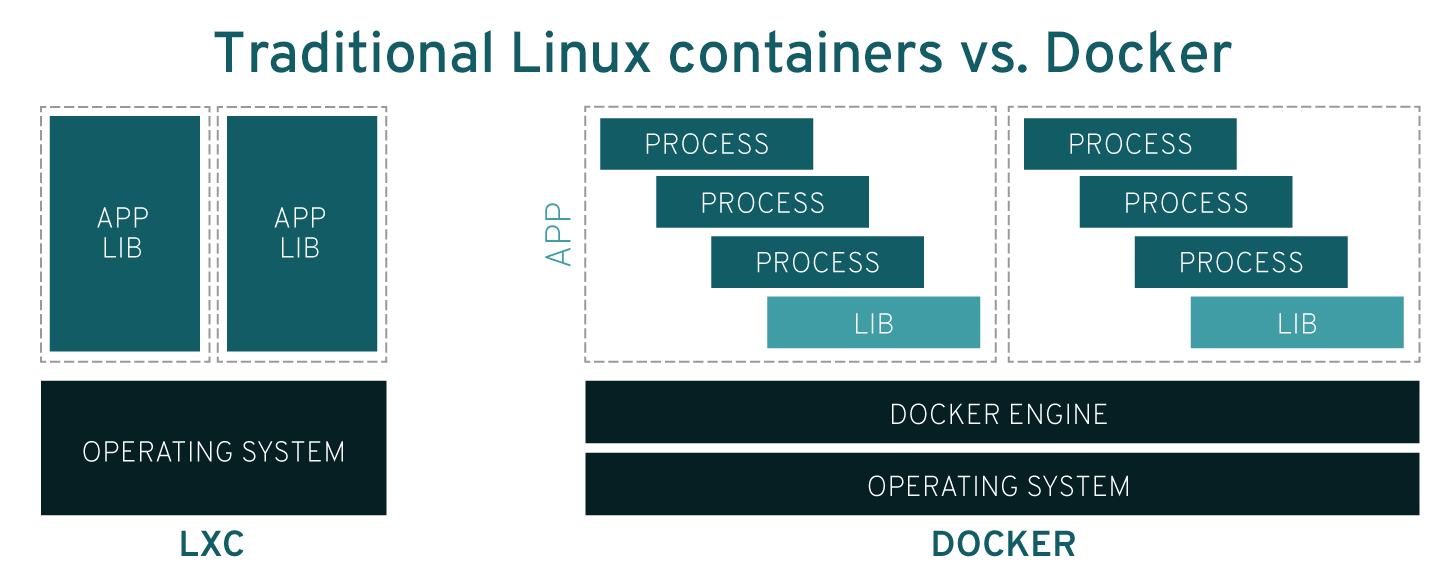
\includegraphics[height=4cm]{img/cap2/traditional-linux-containers-vs-docker_0.png}
\centering

Fonte:~\cite{container}
\end{figure}



\subsection{Docker Swarm}

É uma ferramenta nativa do Docker que permite criar clusters de containers, chamado swarms, o que possibilitam a escalabilidade de recursos de acordo com a demanda(carga)~\cite{turnbullMarc17}
O que possibilita que diversos hospedeiros de Docker estejam inseridos no mesmo pool de recursos, facilitando assim a implantação de containers, uma vez que o Swarm disponibiliza uma API de integração que abstrai grande parte das
atividades necessárias a administração dos conteiners e promove um tipo de tolerancia a falhas


\begin{figure}[htb!]
\caption{Rede de Docker Swarm.}
\label{fig:docker_swarm}
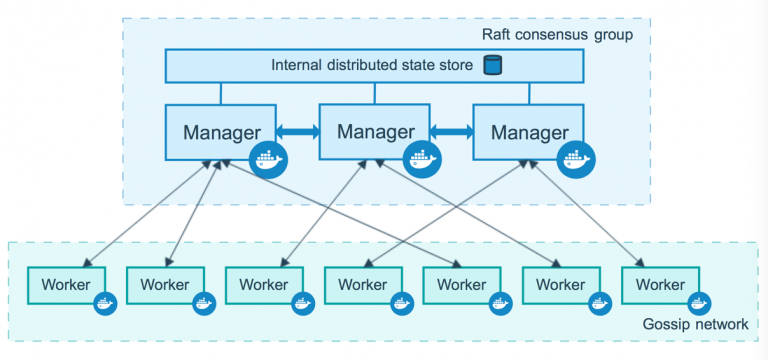
\includegraphics[height=4cm]{img/cap2/docker_swarm.png}
\centering

Fonte:~\cite{container}
\end{figure}


O seu principal objetivo é resolver problemas de gerência de microsserviços, a qual antes eram resolvidos somente com \textit{Kubernets}, uma ferramenta criada pela Google em 2015.
%
Com Docker Swarm, pode-se ter um nó líder que gerenciará a rede, e nós trabalhadores.
%
Um exemplo de rede Docker Swarm pode ser visualizado na Figura~\ref{fig:docker_swarm}.

%\section{Histórico}

\subsection{Arquitetura Monolítica}

Arquitetura Monolítica, é uma arquitetura de desenvolvimento, na qual típicamente , apesar da complexidade dos sistemas ser quebrada ao se utilizar módulos, esses são projetados para a criação de um único executável, o qual possui todos os seus módulos executados em um mesma máquina.
Com o passar do tempo, o sistema cresce e tende a tornar-se cada vez mais complexo, o que gera diversos problemas em sua manutenção, por exemplo temos, a escalabilidade do sistema, que exige que o mesmo seja replicado inteiramente, mesmo que apenas uma parte desse seja necessária na nova instância, aumentando assim os custos.

Com a necessidade de escalabilidade, as arquiteturas de microsserviços obteram sucesso em grandes projetos comerciais como LinkedIn, Google e Youtube.

\begin{figure}[htb!]
\caption{Arquitetura Monolítica X Arquitetura de Microsserviços}
\label{fig:}
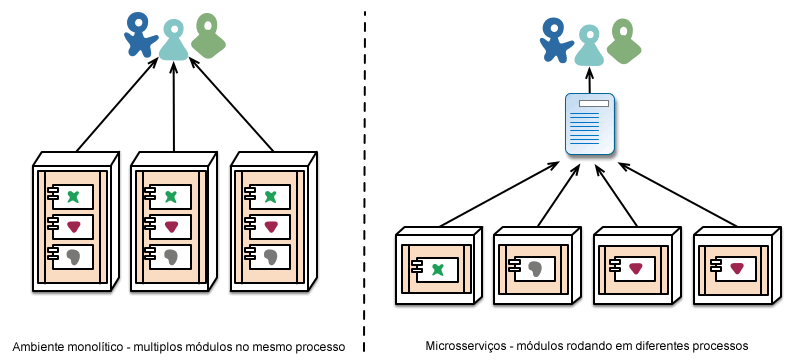
\includegraphics[height=4cm]{img/cap2/monoXmicro.png}
\centering
\end{figure}


%\section{Funcionamento}


\section{Boas práticas}
\begin{itemize}
	\item Não armazenar dados em containers, uma vez que esses podem ser parados, destruidos ou mesmo substituidos, se ncessário armazenar dados deve ser feito em um volume, com o cuidado de evitar que dois ou mais containers escrevam dados em um mesmo volume, o que poderia causar o corrompimento dos dados.
	\item Não criar imagens grandes, já que essas possuirão uma distribuição complexa, uma imagens de possuir apenas as bibliotecas e arquivos necessários para a execução da aplicação ou processo.
	\item Não executar mais de um processo/aplicação em um único container, pois tal comportamento acarretará em aumento da complexidade do gerenciamento e no número de logs.
	\item Não dos endereços IP dos containers, o endereço IP do container pode se alterado quando o mesmo é iniciado e parado. Caso seja necessária a comunicação entre a aplicação ou microsserviço e um outro container, é recomendado o uso de variáveis de ambiente para transmitir o hostname e porta corretos de um container para outro.
\end{itemize}
\cite{boasPraticas}



\section{Principais aplicações}

\subsection{Aplicações Web}

Microsserviços desenvolvidos para web utilizam arquitetura \ac{rest} baseado sobre o protocolo \ac{http}.
É uma boa prática utilizar o corpo com conteúdo da requisição e resposta no formato \ac{json} nas chamadas a uma \ac{api} de microsserviço web~\cite{Nadareishvili2016Aug}.

\subsection{Streaming}
Devido as suas propriedades os microsserviços, possibilitam que operações de streaming(cloud-based) possuam maior elasticidade e escalabilidade do que uma implementação padrão(monolítica), além de possibilitar a redução de custos de operação.\cite{microservicosStreaming}
\subsection{Jogos}

Alguns exemplos de arquitetura de microsserviços para jogos \ac{mmorpg} são as arquiteturas apresentadas por Rudy (Figura~\ref{fig:rudy}), Salz (Figura~\ref{fig:salz}) e a arquitetura escrita por Knowles (Figura~\ref{fig:knowles}).


\begin{figure}[htb!]
  \caption{Arquitetura Rudy, utilizada no jogo Tibia.}
  \label{fig:rudy}
  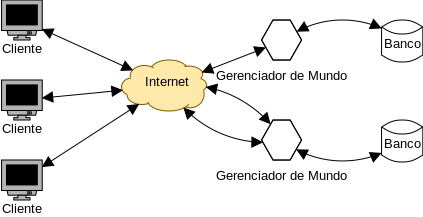
\includegraphics[height=3.5cm]{arquiteturas/rudy.png}
  \centering

  Adaptado de:~\cite{matthiasrudy2011}
\end{figure}


\begin{figure}[htb!]
  \caption{Arquitetura Salz, utilizada no jogo Albion.}
  \label{fig:salz}
  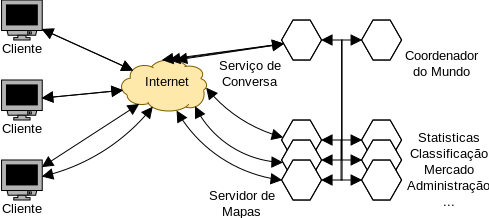
\includegraphics[height=3.5cm]{arquiteturas/salz.png}
  \centering

  Adaptado de:~\cite{albion_online_unite}
\end{figure}%

\begin{figure}[htb!]
  \caption{Arquitetura Knowles, utilizada no jogo Guild Wars 2.}
  \label{fig:knowles}
  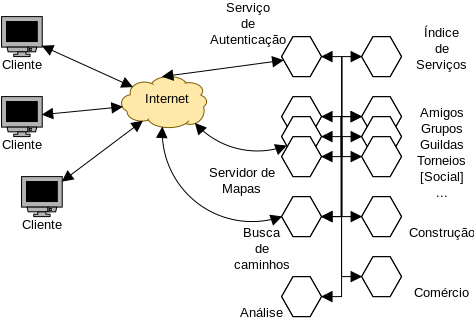
\includegraphics[height=5.5cm]{arquiteturas/knowles.png}
  \centering

  Adaptado de:~\cite{stephenclarkewillson2017}
\end{figure}

A arquitetura Rudy (Figura~\ref{fig:rudy}) é formada por um sistema cliente-servidor monolítico, na qual cada microsserviço individual gerencia um mundo mútuo dos demais gerenciadores de mundo~\cite{matthiasrudy2011}.
%
Essa arquitetura dificulta a escalabilidade, modificações e manutenção~\cite{8169955}, além de segregar a comunidade de jogadores em servidores menores~\cite{matthiasrudy2011}.
%
Inicialmente essa arquitetura foi pensada para ser um sistema Cliente-Servidor monolítico.
%
A arquitetura Rudy é uma arquitetura de microsserviços adaptada de um serviço cliente-servidor~\cite{matthiasrudy2011}.
%
O jogo Tibia\footnote[1]{Tibia: \url{http://www.tibia.com}}, operante sobre essa arquitetura, possui 68 mundos oficiais (Sendo 2 servidores de teste)~\cite{matthiasrudy2011}, com capacidade para 1.050 clientes em cada servidor, na qual encontra-se restringido pelo gerenciador de mundo.



A arquitetura Salz (Figura~\ref{fig:salz}) é formada por diversos microsserviços~\cite{albion_online_unite}.
%
O principal objetivo dessa arquitetura é modularizar o serviço visando melhorar a escalabilidade.
%
Ela é atualmente utilizada no jogo Albion Online\footnote[2]{Albion Online: \url{https://albiononline.com}}.
%
A arquitetura é planejada para funcionar conforme a seguinte especificação\cite{albion_online_unite}:

\begin{itemize}
  \item O mundo é distribuído sobre os vários servidores de mapas. Cada microsserviço gerencia uma região do mundo, denominado \textit{chunk}.
  \item Jogadores mudam a conexão com os microsserviços quando estão posicionados na borda de um \textit{chunk}.
  \item A autorização de acesso aos microsserviços é obtido pelo banco de dados.
  \item O coordenador do mundo é responsável por tudo que seja de escopo global (\textit{e. g.,} Grupos, chat global, guildas, \textit{etc.}).
\end{itemize}

A arquitetura Knowles (Figura~\ref{fig:knowles}) é distribuída em diversos microsserviços, assim como a arquitetura Salz (Figura~\ref{fig:salz}).
%
A diferença em comparação a arquitetura Salz (Figura~\ref{fig:salz}) está na decomposição da arquitetura para outros microsserviços e a conexão direta entre esses microsserviços e o cliente.
%
O principal objetivo dessa arquitetura é facilitar a manutenção e desempenho de reinicialização do macrosserviço~\cite{stephenclarkewillson2017}.
%
Guild Wars 2\footnote[3]{Guild Wars 2: \url{https://www.guildwars2.com}} é um jogo que executa sobre a arquitetura Knowles.
%
Ele é popularmente conhecido por ter seus serviços sempre ativos, visto que a arquitetura possibilita desativar pequenos pedaços do serviço para manutenções básicas e a sua reinicialização é rápida para manutenções críticas.

\chapter{Casos Comentados}
\label{cap2}

\section{Walmart}

\section{Spotify}

\section{Amazon}

\section{Guild Wars 2}

\chapter{Análise}
\label{cap3}

\section{Método de deploy}

\section{Arquitetura obtida}

\section{Análise sobre a arquitetura obtida}

\chapter{Conclusão}
\label{cap4}

Conclusão


%\section*{Agradecimentos}

AGRADECIMENTOS


%---------- Referências ------------------------------------
\renewcommand{\bibname}{Referências}
\bibliographystyle{pkg/abnt-alf}
\bibliography{refsTcc}

%---------- Apêndice ---------------------------------------
%\appendix
%\chapter{Apêndice: Cronograma}
\label{ap:crono}

CRONOGRAMA


%-----------------------------------------------------------
\end{document}
